\clearpairofpagestyles
\renewcommand{\pagemark}{{\usekomafont{pagenumber}{\thepage\ / \pageref{LastPage}}}}
\ohead*{\vspace{-1cm} 游戏设计作品集 \hfill}
\ofoot*{\pagemark}
\pagenumbering{arabic}
\setcounter{page}{1} %%% This is only to be included in the first content file to restart the page numbers using a different format %%%

\NewChapter{三个字}

\quote{在张望,有太多迷茫,我想起夕阳下的奔跑。}{《万万没想到》}

回忆童年时光,我们总是可以想起那些阳光明媚的日子,和小伙伴一起度过的美好时光。在夕阳下,我们总是不肯回家,跑得满身臭汗被父母臭骂一顿再吃上香喷喷的晚饭。童年中最火爆的游戏之一就是大家一起奔跑的多人游戏——鬼抓人!“三个字”则是鬼抓人最受欢迎的变种!

“三个字”抓人游戏的规则可以简化为如下:

\begin{enumerate}
    \item 游戏分为两个阵营——狼和羊,狼的胜利目标是在规定时间内抓到所有羊,羊的目标是存活;
    \item 狼抓到某只羊后,该羊加入狼阵营;
    \item 羊可以大喊“三个字”冻结自己,冻结自己后无法移动,狼无法抓被冻结的羊;
    \item 没有被冻结的羊可以解冻其它冻结的羊;
    \item 最后一只没冻结的羊不可以冻结自己。
\end{enumerate}

\section{创作背景}
游戏创作于 2022 年 11 月,是清华大学互动媒体设计与技术专业开设的游戏开发课课程大作业。作业要求两人一组,开发一款基于Skynet多人游戏网络框架的多人在线游戏。当时多个DDL来临,团队二人压力很大,于是我们决定放弃那些对抗、战斗的题材,想要利用童趣和回忆唤起大家孩童时期的快乐时光。我们思考了多个童年游戏原型,比如“老鼠偷油”、“一二三木头人”和“三个字”等,均聚焦于使用大脑系统一的游戏,想利用简单直接的刺激带给玩家快乐。

最终我们改编了“三个字”,做成了四人在线战术非对称捉迷藏游戏,\textbf{游戏因较高的完成度和游戏性最终在试玩会被腾讯、清华老师组成的评审会授予“项目管理大师奖”}。

\begin{figure}[H]
    \centering
    \includegraphics[width=0.8\textwidth]{Images/三个字/sgz.png}
    \caption{三个字\ 游戏封面}
\end{figure}

\section{设计思路}
在改造为电子游戏的过程中,我们采用同心开发的方式,进行了数值层面的快速迭代。最终确定一局游戏时间为90秒。同时,童年时如果狼是跑步速度较慢的同学,羊队往往会以极大的优势获得胜利。所以,我们直接给狼赋予了更快的移动速度和冲刺速度。但是,小时候羊队往往会有高手,在层层环绕的树林和建筑中,利用假动作和横移速度利用地形摆脱狼的追击。所以,我们赋予羊更高的横向移动速度,力图还原那种勾心斗角的抓人体验。

\begin{figure}[H]
    \centering
    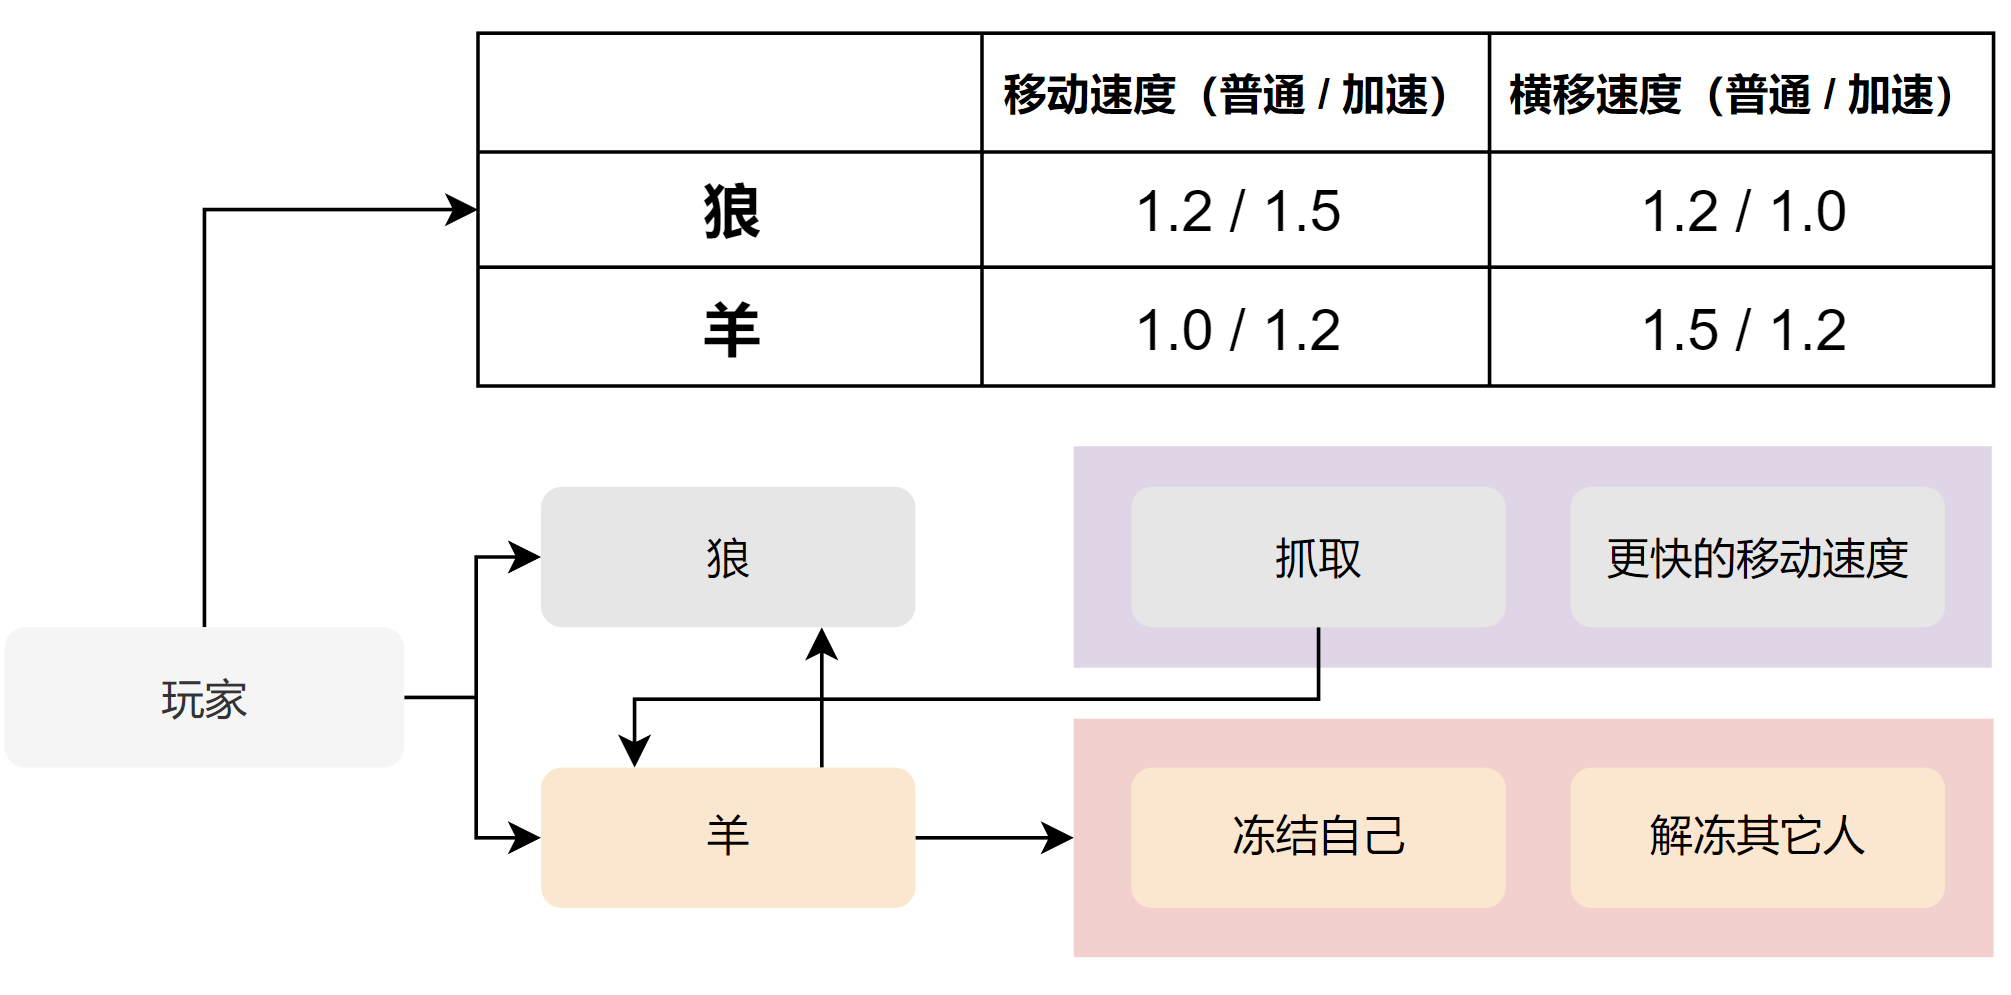
\includegraphics[width=0.9\textwidth]{Images/三个字/sgz_division.png}
    \caption{三个字\ 游戏角色设计}
\end{figure}

而战术竞技最重要的一环则是关卡设计。一方面为了平衡羊队和狼队实力,一方面为了给予不同玩家不同的游戏体验。我在设计关卡时,有意识地将地图划分为四个板块,并利用贯穿地图的道路给予玩家动线提示。而最终设计因为技术和时间等因素没有完全复刻,但基本已经形成了不同玩家在不同区域内通过发挥自身优势达到不同乐趣的游戏体验。

\begin{figure}[H]
    \centering
    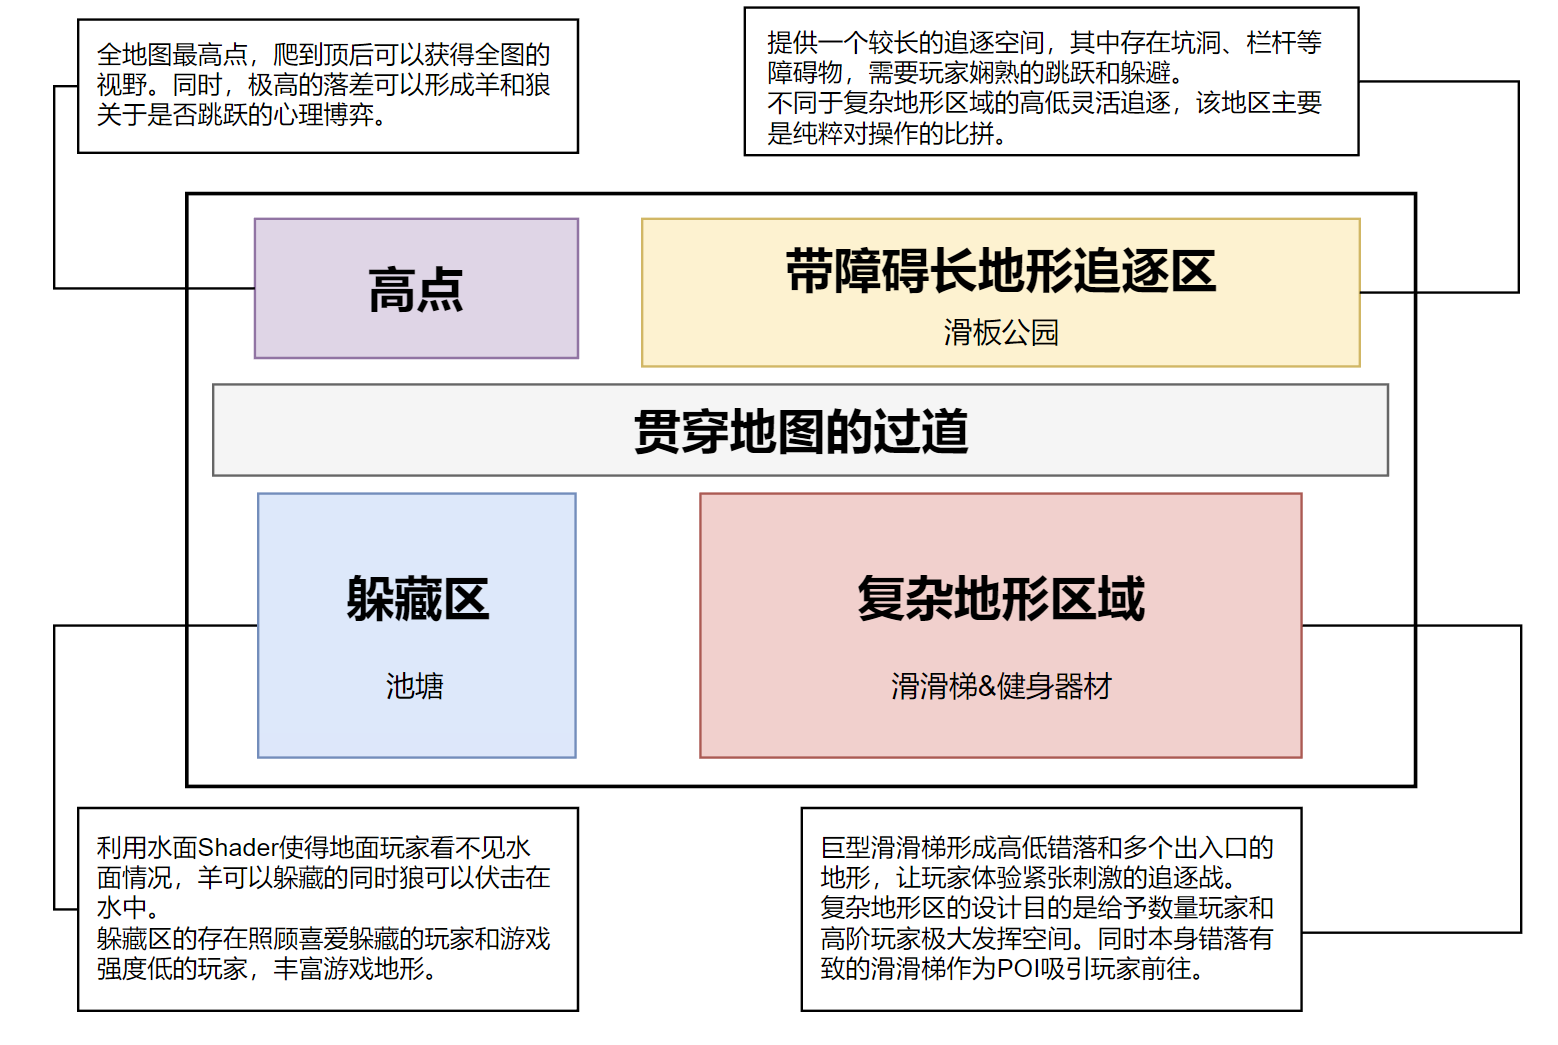
\includegraphics[width=0.9\textwidth]{Images/三个字/sgz_level.png}
    \caption{三个字\ 关卡设计}
\end{figure}

\section{游戏演示}
因为游戏最终租用的云服务器已经到期,目前游戏已无法正常进行线上模式,通过图片、视频、推送等形式展示。


\begin{figure}[H]
\centering  %图片全局居中
\subfigure[玩家登陆界面]{
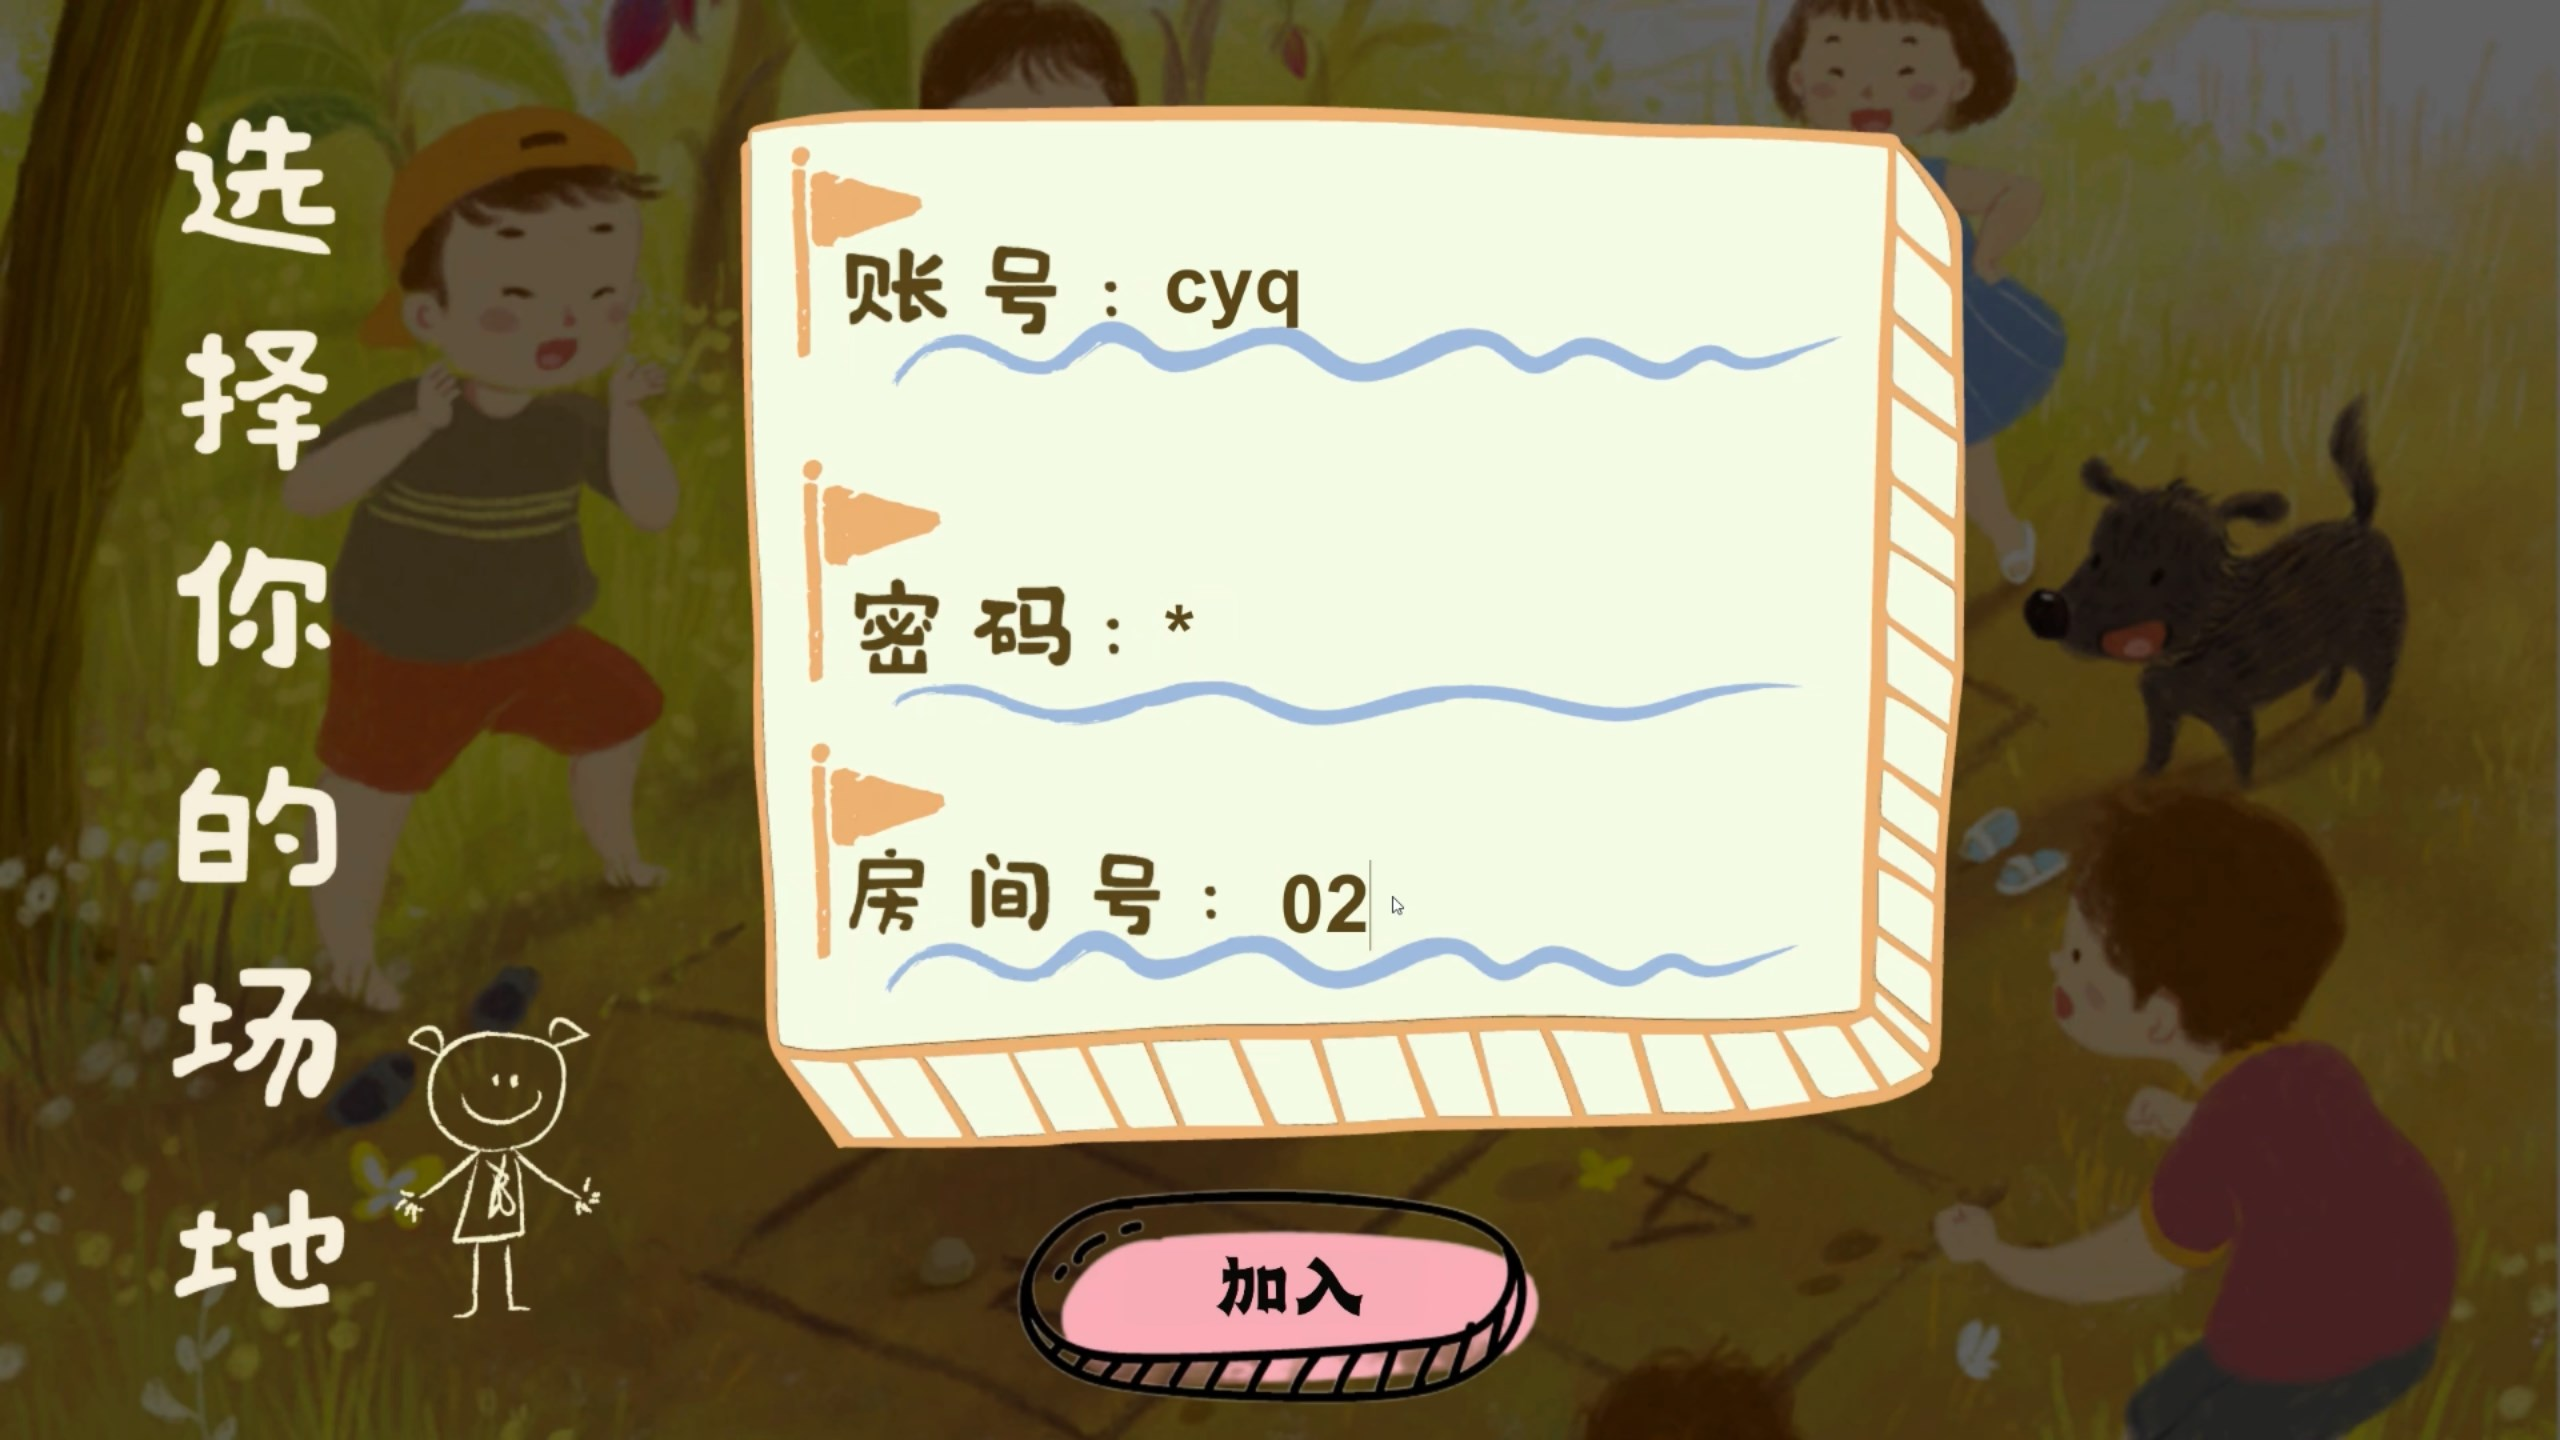
\includegraphics[width=0.45\textwidth]{Images/三个字/sgz5.jpg}}
\subfigure[游戏准备大厅]{
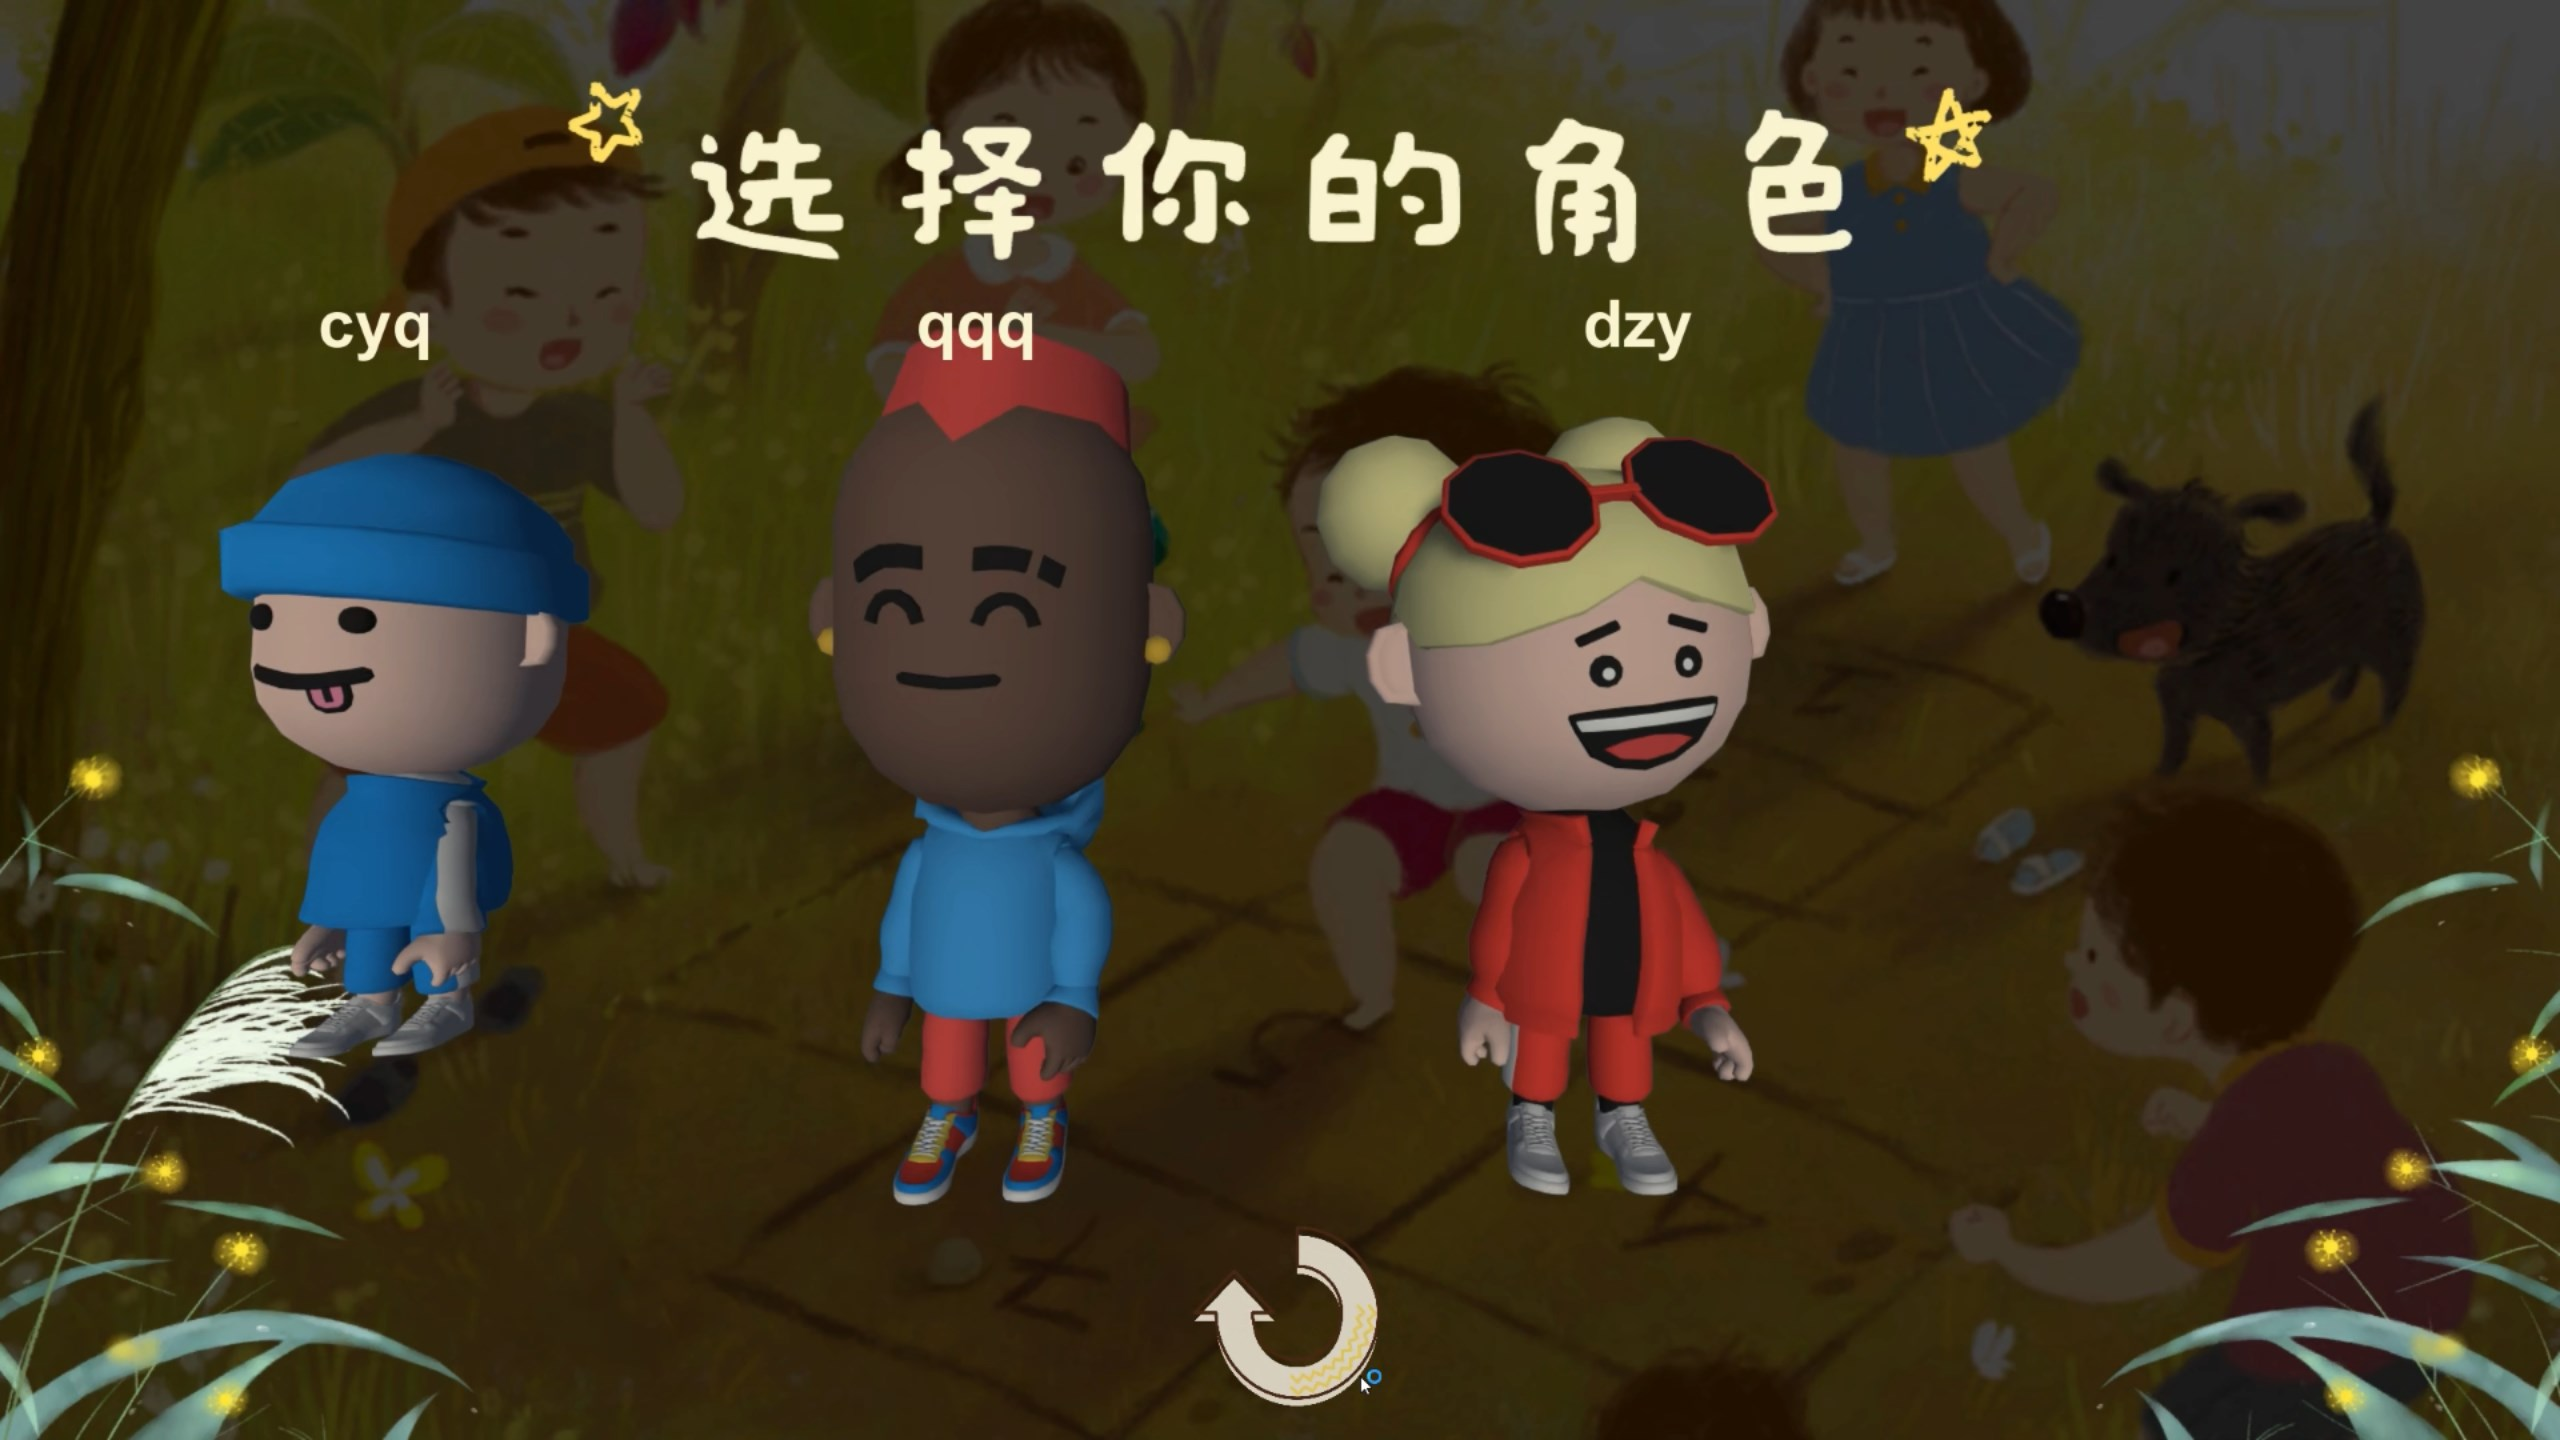
\includegraphics[width=0.45\textwidth]{Images/三个字/sgz1.jpg}}

\subfigure[游戏内操作指引]{
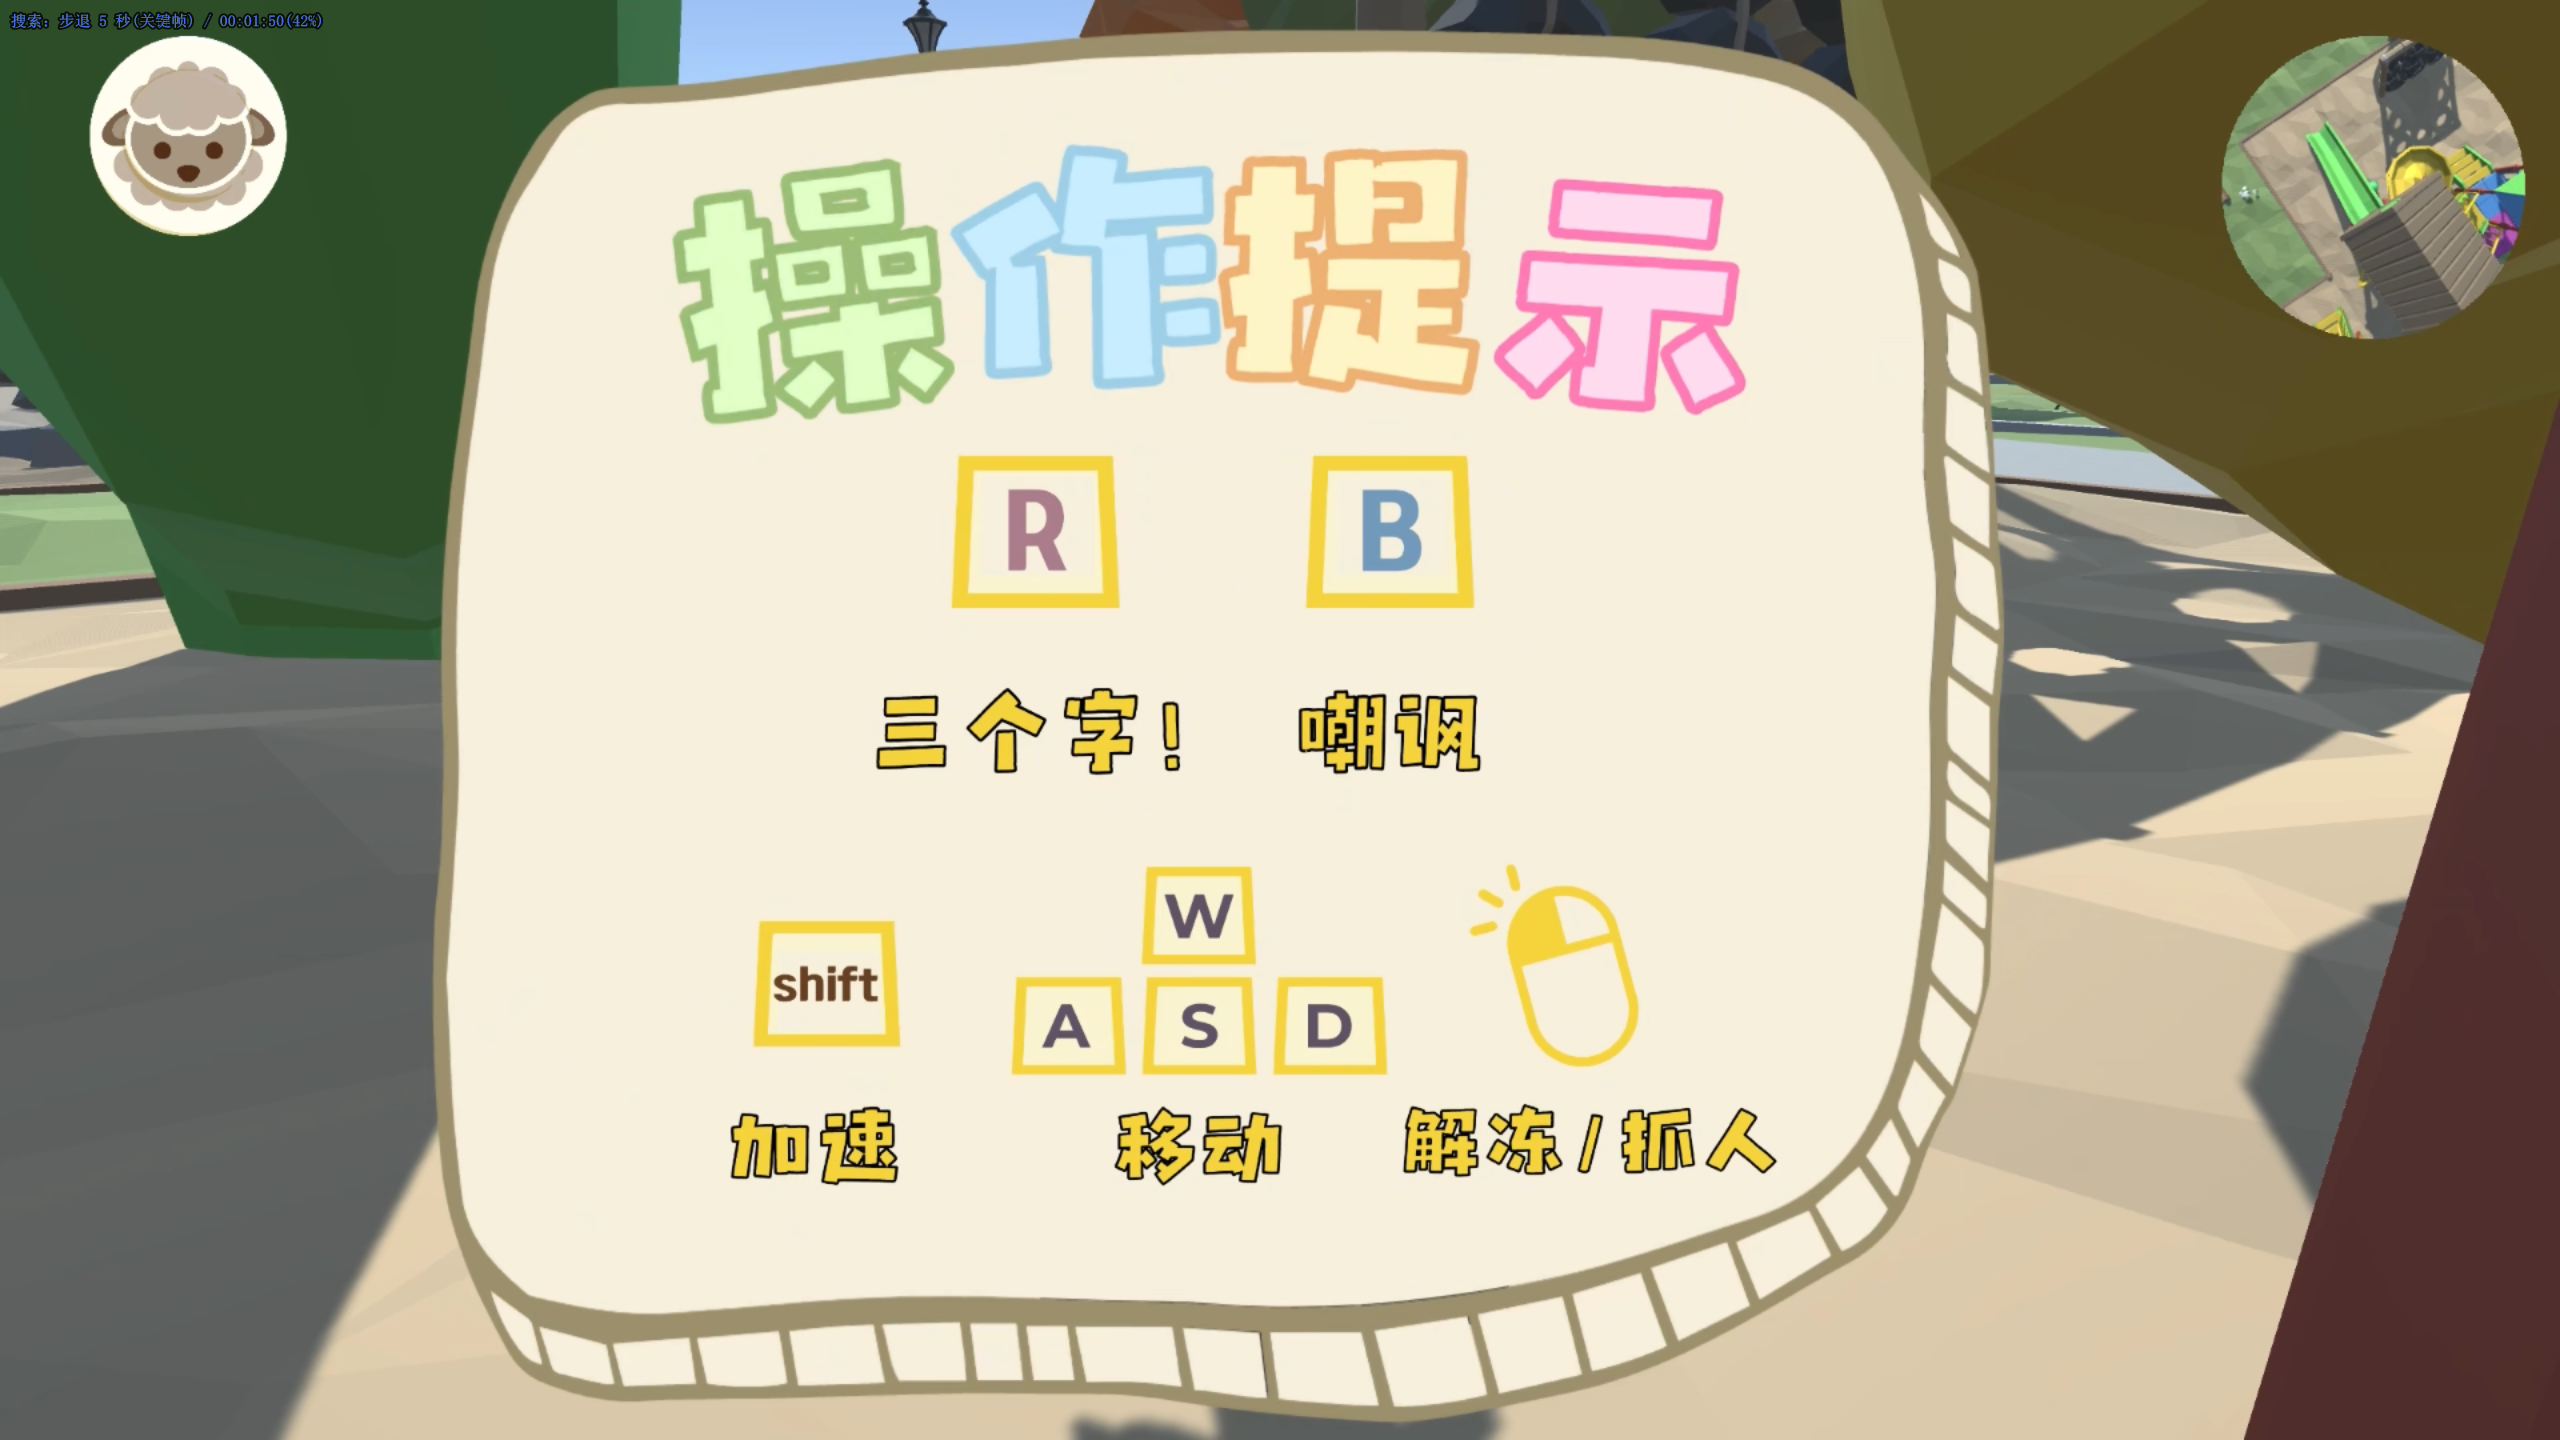
\includegraphics[width=0.45\textwidth]{Images/三个字/sgz2.png}}
\subfigure[游戏实机画面]{
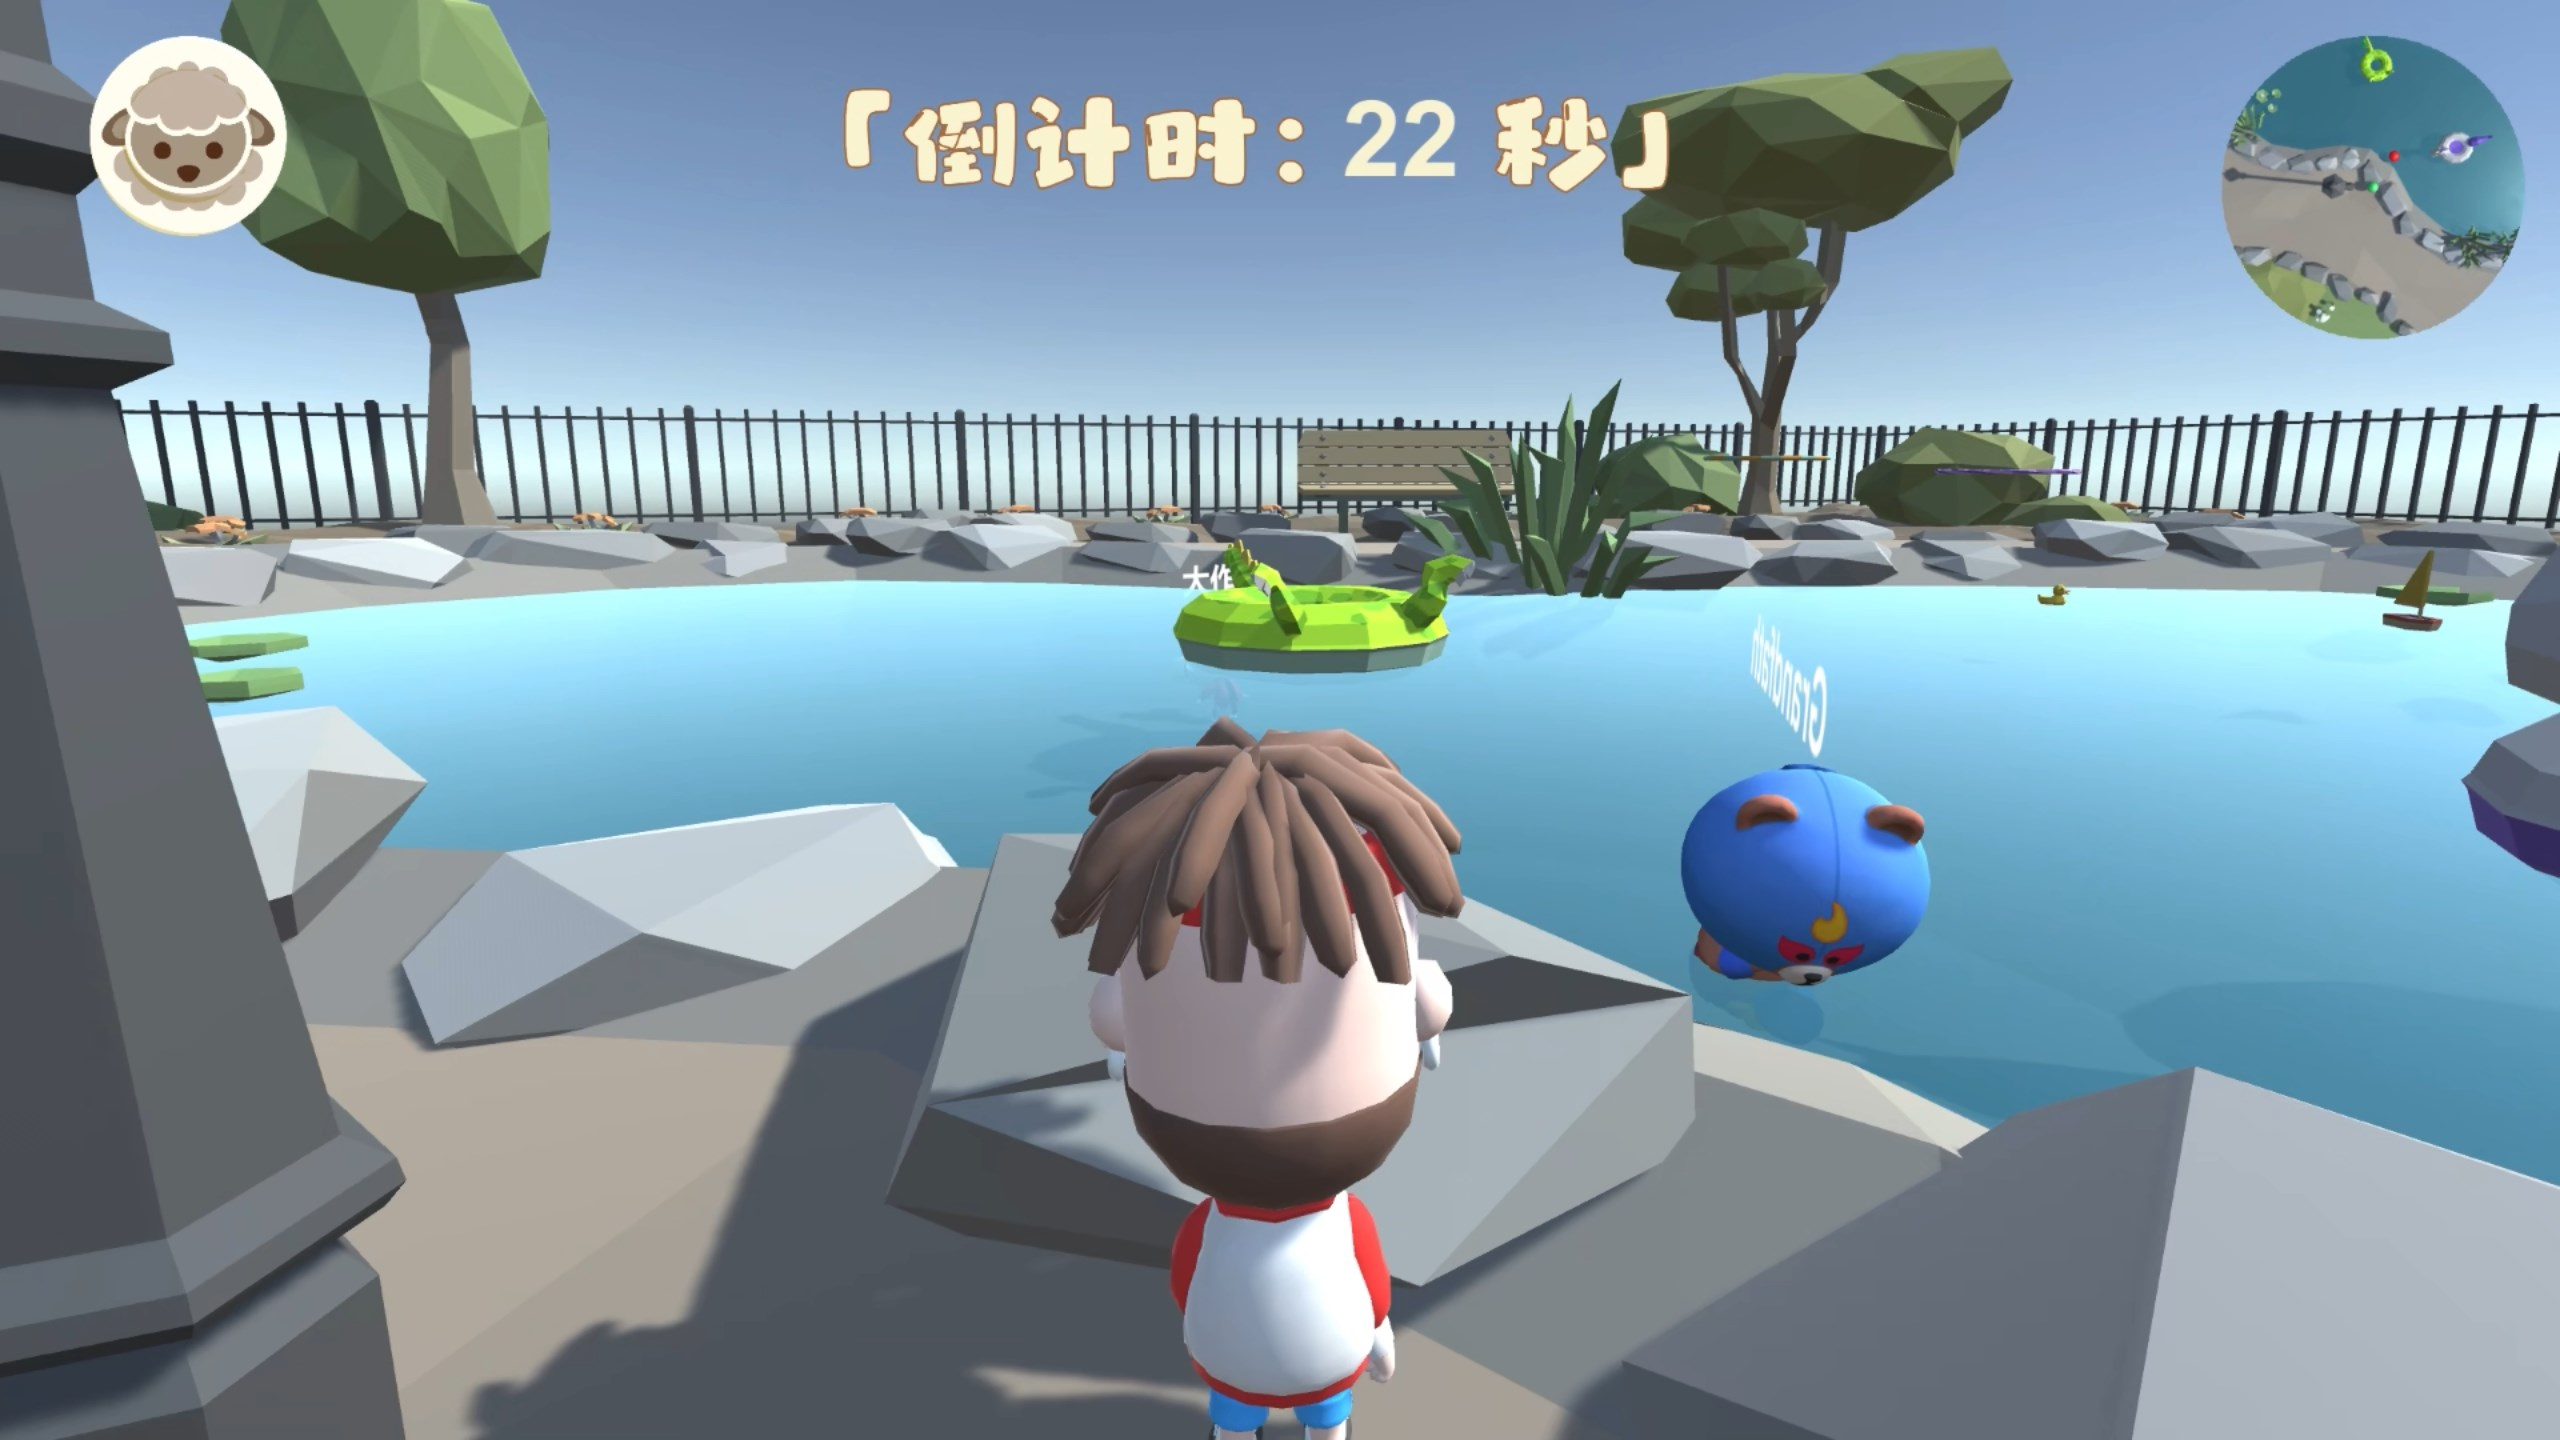
\includegraphics[width=0.45\textwidth]{Images/三个字/sgz3.jpg}}
\caption{三个字\ 游戏画面}
\end{figure}




\begin{itemize}
    \item \textbf{试玩视频:}  \href{https://www.bilibili.com/video/BV1W84y1G7Wa/?vd_source=ead0ac501dfae814e19fd7d9f376d92d}{Bilibili视频}
    \item \textbf{推送链接:}  \href{https://mp.weixin.qq.com/s/4vQjfRlGlBNg2u_2wrgUdw}{SIGS IMDT 公众号} 
\end{itemize}